\section{Introduction}
% Just here to show that we can put todo notes in the doc, can be removed later
% Let's do things\todo{sup}

% Just here to show how listings are done in this template, can be removed later
% \begin{lstlisting}
% test
% fiets
% test
% \end{lstlisting}

% Short abstract introduction here about this section (can be done when finished)

\subsection{Background}
% What is SeaDataCloud's exact problem? Make the problem clear so that our solution fits the problem. Try to look at it from all angles, like an os3 teacher would
% SeaDataCloud is a distributed infrastructure to manage large and diverse sets of data about seas and oceans. This Pan-European network offers data access to support scientific workflows which varies from climate change prediction to offshore engineering\cite{sdc}. SeaDataCloud has 8 institutes with over 100 data centers, with the aim to make research data available to scientist.

% Different independent organizations push data into this infrastructure which are then automatically and manually curated to ensure correct data formats. A PID (Persistent Identifier) is then assigned when it’s stored in the catalog. This PID ensures that the data can be identified, independent of its location in the infrastructure\cite{icn-survey, icn-bd}.

% Data consumers pull data from this catalog by the means of point-to-point connections (IP), where every data request from the consumer are answered with a data transfer from the source (the producer). This approach can potentially cause congestion and delays with many data consumers. Named Data Networking (NDN) is a data centric approach where unique data, once requested, is stored on intermediate locations. Consecutive requests for that unique data object are then made available by these intermediate locations (caching). This approach distributes traffic load more efficient and reliable compared to point-to-point connection oriented techniques\cite{ndn}.

SeaDataClouds current model is a centralized solution, as the current cache duplicates the entire data repository. This can cause a lot of congestion with many users and does not distribute load efficiently. 
SeaDataCloud proposed a model to introduce NDN, as seen in figure \ref{fig:sdc_ndn}. With NDN, data is cached at intermediate routers which brings the data closer to the consumer. The data hosting organization pushes the object in NDN, where the PID resolver does the translation from PID name to a NDN name (to be used withing NDN) and inserts the data in NDN. After the object has been inserted in NDN, the data consumer then can request the object from the NDN network. 

Their proposed model currently only supports one PID provider also referred to as PID type. Interoperability of different PID types has not been realized yet. 

\begin{figure}[H]
\centering
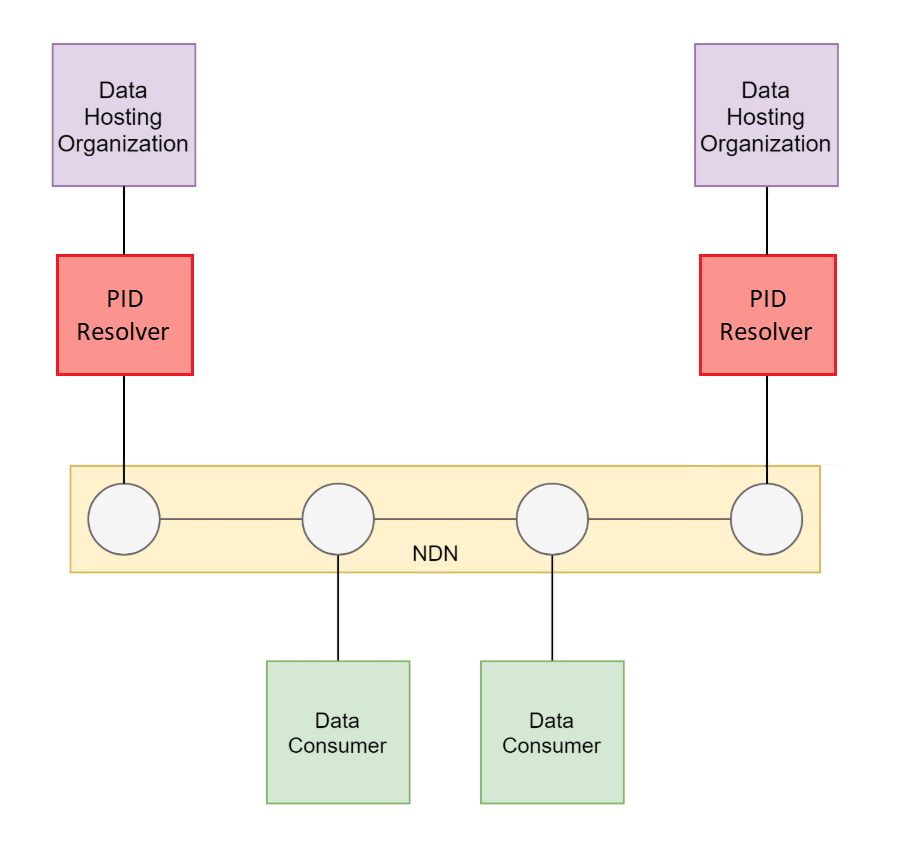
\includegraphics[scale=0.5]{Images/sdcrp2.png}
\caption{SeaDataClouds proposed NDN model.}
\label{fig:sdc_ndn}
\end{figure}

\subsection{What is a PID?}
Shortly after the introduction of the World Wide Web (WWW), Tim Berners Lee (its' creator) proposed in the Internet Engineering Task Force (IETF) to use the Uniform Resource Identifier (URI) as the naming scheme for identifying 
contents on the Web. This proposal got rejected by IETF, due to the fact that it does not allow users of the Web to change the URI of the Web contents when moving the Web contents to another location. This lead to the use of Uniform Resource Locators (URLs) as the naming scheme to identify Web content.
 
The use of URLs was no issue at the early stages of the Web, but after a while users of the WWW began to experience the problem of a broken link, or the  so called "link rot" problem, 
where a user fails to retrieve the (a digital object) Web content by its URL, 
due to the fact that the location of the Web content has been changed \cite{icn-bd, ark-id}. 
Web contents refer to digital resources or so called digital objects.

Therefore the first Persistent Identifier (PID) systems emerged in the mid-1990s shortly after the introduction of the Web itself. 
A PID is a long-lasting, permanent reference to a digital resource. Traditional identifiers, such as the bibliographic identifier ISBN will not be interpreted as a 
hyperlink by Web browsers. For example the string \texttt{ISBN 951-45-9942-X} has to be expressed as a HTTP URI in the form of \texttt{http://urn.fi/URN:ISBN:951-45-9942-X} to be a persistent link to the resource.  
When using a PID, a user who requests the digital resource can trust that the appropriate digital resource is retrieved, 
even if the location where it resides has been changed \cite{pid-oview}.

\subsection{What is NDN?}
When the internet was conceived it was designed for host-to-host communication. This means that in order to retrieve data, a host needs to retrieve its data from a single source. Nowadays the internet is increasingly data-oriented rather than host-oriented. For example growth in digital media and social media traffic. With many users requesting the same video, congestion becomes a problem. The geographical location sits on top of that problem, since data needs to cross distance as well, resulting in latency.

The primary use-case of the internet has become data distribution. Solving distribution problems with a host-to-host communications network is complex and error prone. The focus of NDN \cite{ndn-summary} is to change the communication model by removing the restriction that packets can only name communication endpoints. In an NDN network the endpoint is a chunk of a video, book or data set.

NDN’s minimal functionality includes support for consumer-driven data delivery, built-in data security, and use of in-network caching. This model provides support for scaling data, balancing data flows for congestion control and retrieving data via multiple paths. This is done by routing packets based on their name rather than destination. When data is sent across the NDN network, it's cached at intermediary hops. Consecutive request for the same data can then be provided by these local in-network caches. The data integrity can be verified via cryptographic hashes. Therefore, this data-oriented model mediates congestion and latency compared to host-oriented models. Section \ref{overview-ndn} provides a more detailed explanation of NDN.

\subsection{Related work}
% Related work summary, only stuff that's directly relevant for our research. Other references can be made later by simply mentioning them. Avoid summarizing related work in too much detail, keep it clear and concise. We need to show our contribution, not what others did.

\subsubsection{PID interoperability}
In 2014, Andreas Karakannas researched the efficiency of ICN (Information Centric Networking) for delivering big data with PIDs. PIDs are used in big data infrastructures to identify digital content and research data. An example of a PID type is DOI (Digital Object Identifier), which is used for object identification. In section \ref{pid-types} we will explain more about PID types. The research proposed a mapping architecture for resolving PIDs to ICN names and evaluated the efficiency of in-network caching when delivering big data objects. Andreas proposed to use a PID to NDN mapping server for every PID type instead of doing the translation on the clients browser. For the latter the researcher states that translation of a PID to NDN name will  be  highly  depended  on  the  clients  NDN browser  which  will  need  to  be  updated  every  time  new  rule  would  be  appeared  or changed \cite{icn-bd}.
%The research results showed that in-network caching can offer significant performance benefits, when the cache size of the network elements that perform in-network caching is bigger than the Big Data object size. 

In 2017, Rahaf Mousa researched the fetching and sharing of DOI objects with information centric networking paradigm such as NDN. 
%(Named Data Networking). 
%For this, the effect of ordering a group of objects in ascending or descending order according to their sizes before requesting them one by one was studied. The research concluded that these ordering methods showed that the methods proposed can dramatically influence the fetching performance of objects from NDN networks. 
The researchers approach focused only on DOI identified objects within NDN networks, which was possible, and states that there are many other different PID systems that can also be integrated. Furthermore, the research states that difference in NDN naming of different PID providers must be taken into account, such that the correct prefix is used within NDN to identify specific PID types within the NDN network. For example using the prefix "doi/" within NDN for DOI identified objects. 
%By doing this,   
In the researchers model, the translation happens at the consumers browsers and a consumer has the choice to either request the digital object by its NDN name or PID \cite{ndn-app-aware}.
%Rahaf Mousa also experimented with cache replacement methods to evaluate which method gives the most performance gain and found that LRU (Least Recently Used) cache replacement strategy gives the highest performance with the proposed ascending ordering according to size method \cite{ndn-app-aware}.

Zhiming Zhao et al. worked further on the research done by Andreas Karakannas and Rahaf Mousa and proposed an architecture to map PIDs onto the naming scheme of NDN. Their proposed solution is called NDN-as-a-service for PID data objects (NaaS4PID) and support one PID type. This solution is composed out of three key components \cite{icn-resteam}:
\begin{itemize}
  \item PID2NDN gateway; primarily responsible for resolving PIDs to NDN names.
  \item NDN4PID router image; an NDN node that implements a virtualized NDN router.
  \item NDN4PID manager; automates the management of the NDN overlay in cloud or e-infrastructure.
\end{itemize}

Chengyu Fan et. al.
-Almost same model as us, catalog instead of GW

Catherine Olschanowsky et. al. 
-Uses translator
-CMMAP/CMIP climate modeling scheme filename translation to NDN by replacing all "." for "/". and just like Rahaf stated that difference in NDN naming of different PID providers must be taken into account, using the model-specific naming scheme as a prefix in NDN instead of a PID type provider, in this case use /CMMAP as a prefix in NDN for routing data.   



\subsubsection{Planning an NDN network}
% NDN planning - how to plan a network - book: network analysis, architecture and design, explain the method
James McCabe's "Network Analysis, Architecture, and Design" \cite{mccabe2010network} book offers a systems methodology approach towards network design. Not only network components are taken into account for design but also the services it supports along with the users needs. The approach is described in McCabe as "seeing the network part of a larger system, with interactions and dependencies between the network and its users, applications and devices". The methodology put forward by McCabe is to design a network based on several inputs and outputs:
\begin{itemize}
    \item Analysis: What do users/services require? How are the relationships composed between these components?
    \item Architecture: Which technology and topology choices support the users/services needs? Based on this, create high-level, end-to-end structure of the network.
    \item Design: Determine the physical detail of the architecture based on output of previous steps.
\end{itemize}

The input and outputs used in this method are intended to be iterative and by no means define a final architecture design. This is due to the fact that requirements, technology and behaviour can change and with that the network design. Section \ref{overview-mccabe} provides a more detailed overview of this method and section \ref{method-planning} describes how it's applied for this research.
% discuss RMA from book

% An NDN network uses routers, bandwidth and other resources to provide its users with a service. Therefore, the methodology described in McCabe can be used to plan an NDN network as well. However, traditional network designs focus on capacity planning, which is over-engineering the amount of network capacity needed. In NDN, with in-network caching, network traffic is distributed by design. Therefore, McCabe's systems methodology will be used, but slightly adapted to NDN. 

% TOSCA - maybe skip this here, almost no academic related work

\subsubsection{Scale an NDN network}
ICN is the common architectural idea of forwarding packets based on their name rather destination (TCP/IP). Research done by Karakannas \cite{icn-bd} concluded that NDN was the only ICN approach that published a specification and workable software to experiment with. As of writing this report, we concluded that this conclusion still holds up. Therefore, this research used NDN for experimentation.

% NDN scaling - how to serve many users - large testbed paper, summarize their findings - named data networking on a router
NDN is relatively new and thus not much is known yet about the performance in different scenarios. In order to plan a network, it first would be useful to know what works and doesn't work for NDN. Large NDN testbeds are still rare. However, there is sufficient research available that focused in on particular design choices of NDN. 

Research done by Lim et al. \cite{lim2018ndn} at a large existing testbed located in the USA \cite{ndn-testbed-status} highlighted a few lessons learned. Lim et al. setup the first intercontinental NDN testbed with the intent to see the benefits for big science (big data). They implemented a name translator for climate-science data, which translates CMIP files to an NDN compatible name. They concluded that NDN provided performance improvements compared to classical climate data delivery techniques based on TCP/IP.

The conclusions of Lim et al. correlates with research done by Shannigrahi et al. at the USA-based large hadron collider network \cite{shannigrahi2015named}. Shannigrahi et al. achieved a 71\% reduction in the average delay per data chunk compared to a no-caching case. Shannigrahi et al. conducted NDN caching simulations \cite{shannigrahi2017request}. They concluded that a small cache of several gigabytes already reduces network load. However, as expected, increasing the cache towards 1TB reduced network even more. But this reduction of load wasn't proportional with the cache size. They concluded in their research that a 1GB NDN cache at the edge of the NDN network can already significantly improve data distribution and reducing the network load from servers. The average file size in use was 1.3GB.

% which cache strategy to use? andreas research + mousa

% downtime of routers must be avoided due to cache rebuild (somewhere in a paper)


\subsection{Research question}
% Based on the use-case and related work, what is it that we will research and why? What is it that we want to answer?
In this section we will formulate our research question based on SeaDataClouds proposed model to use PIDs to uniquely identifiying digital objects and use NDN to reduce latency for the user and reducing congestion in the cloud.

For using PIDs in NDN, we have to look into PID to NDN translation to make PIDs interoperable in the NDN network. Therefore the following research question is formulated.

\begin{itemize}
	\item How to make the Persistent Identifier (PID) and NDN (Named Data Networking) namespace interoperable?
\end{itemize}

As SeaDataClouds proposed solution only supports one PID type at the moment, we will look into supporting different PID types and find a way which is feasible to implement future PID types easily. This will be answered with the following subquestions.
\begin{itemize}
    \begin{itemize}
	    \item How to support different PID types?
	    \item How to incorporate extensibility for future PID schemes?
	 \end{itemize}   
\end{itemize}

As SeaDataClouds current model is a centralized solution, which can cause a lot of congestion with many users and does not distribute load efficiently and reliably, their proposed model incorporstes NDN to overcome the issues of traditional host-to-host oriented techniques. Therefore we will be looking into introducing NDN in SeaDataCloud. To achieve this, the following research question needs to be answered.   
\begin{itemize}
    \item How to plan and scale an NDN network?
\end{itemize}

An important aspect is to efficiently use an NDN network in such a cloud infrastructure by scaling up or down to adapt to the load. To accomplish this, 
%we will look into 
%To plan and scale an NDN network, 
the known NDN scaling problems must be brought to light. Furthermore we will look into methods to make it possible to plan and scale an NDN network by deploying (orchestrating) components of an NDN network in a SDN fashioned way.
\begin{itemize}
    \begin{itemize}
	    \item Which NDN scaling problems are known?
	    \item Which method can be used to plan an NDN network?
	    \item How to deploy an NDN network in a scalable way?
	\end{itemize}
\end{itemize}


\subsection{Scope}
% What will we do and what will we skip? Based on what's already done in related work and our research question
The use case that SeaCloudData offers is suitable to further research and improve interoperability of different PID types in NDN and planning and scaling such an NDN network. In order to accommodate multiple data producers, for which each has their own PID scheme, a custom tailored mapping needs to be made which will be derived and from the related work done earlier and improve our model by tackling the issues the researches came across. Support for future PID types with different naming schemes should be asily extensible, therefore we will also look into a solution which makes this possible. 

This also requires to look into the design patterns of such a deployment where scalability and automated provisioning are key requirements. For this, we will look into different orchestration solutions like Kubernetes and TOSCA for managing a NDN network in a Software Defined Networking (SDN) fashion.

\subsection{Report structure}
After having introduced the reader to the concepts and related work of our researched subjects, this paper starts with a technical overview of the technology being used in section \ref{tech-oview}. In this section we will describe PIDs, NDN, McCabem, TOSCA and virtualization in more depth and more detail.
The paper continues by describing our methodology, which includes showing our proposed model which describes how interoperability is achieved. Furthermore this section will bring the attention of how to plan a NDN network by using orchestration tools such as McCabe and TOSA and how NDN scalability is achieved. 
After the aforementioned section we will get to the results section to show the results we got from the experiments based on our methodology.
The discussion section then follows to discuss difficulties we came across during our research and what advice can be given to the reader.
Finally we enforce the value of this research by concluding our findings and end our research by giving insight in future work for the readers to think about and perhaps getting picked up by other researchers. 

% To guide the reader into what's to come, can be done only when whole report is done